% Options for packages loaded elsewhere
\PassOptionsToPackage{unicode}{hyperref}
\PassOptionsToPackage{hyphens}{url}
\PassOptionsToPackage{dvipsnames,svgnames,x11names}{xcolor}
%
\documentclass[
  letterpaper,
  DIV=11,
  numbers=noendperiod]{scrartcl}

\usepackage{amsmath,amssymb}
\usepackage{lmodern}
\usepackage{iftex}
\ifPDFTeX
  \usepackage[T1]{fontenc}
  \usepackage[utf8]{inputenc}
  \usepackage{textcomp} % provide euro and other symbols
\else % if luatex or xetex
  \usepackage{unicode-math}
  \defaultfontfeatures{Scale=MatchLowercase}
  \defaultfontfeatures[\rmfamily]{Ligatures=TeX,Scale=1}
\fi
% Use upquote if available, for straight quotes in verbatim environments
\IfFileExists{upquote.sty}{\usepackage{upquote}}{}
\IfFileExists{microtype.sty}{% use microtype if available
  \usepackage[]{microtype}
  \UseMicrotypeSet[protrusion]{basicmath} % disable protrusion for tt fonts
}{}
\makeatletter
\@ifundefined{KOMAClassName}{% if non-KOMA class
  \IfFileExists{parskip.sty}{%
    \usepackage{parskip}
  }{% else
    \setlength{\parindent}{0pt}
    \setlength{\parskip}{6pt plus 2pt minus 1pt}}
}{% if KOMA class
  \KOMAoptions{parskip=half}}
\makeatother
\usepackage{xcolor}
\setlength{\emergencystretch}{3em} % prevent overfull lines
\setcounter{secnumdepth}{-\maxdimen} % remove section numbering
% Make \paragraph and \subparagraph free-standing
\ifx\paragraph\undefined\else
  \let\oldparagraph\paragraph
  \renewcommand{\paragraph}[1]{\oldparagraph{#1}\mbox{}}
\fi
\ifx\subparagraph\undefined\else
  \let\oldsubparagraph\subparagraph
  \renewcommand{\subparagraph}[1]{\oldsubparagraph{#1}\mbox{}}
\fi

\usepackage{color}
\usepackage{fancyvrb}
\newcommand{\VerbBar}{|}
\newcommand{\VERB}{\Verb[commandchars=\\\{\}]}
\DefineVerbatimEnvironment{Highlighting}{Verbatim}{commandchars=\\\{\}}
% Add ',fontsize=\small' for more characters per line
\usepackage{framed}
\definecolor{shadecolor}{RGB}{241,243,245}
\newenvironment{Shaded}{\begin{snugshade}}{\end{snugshade}}
\newcommand{\AlertTok}[1]{\textcolor[rgb]{0.68,0.00,0.00}{#1}}
\newcommand{\AnnotationTok}[1]{\textcolor[rgb]{0.37,0.37,0.37}{#1}}
\newcommand{\AttributeTok}[1]{\textcolor[rgb]{0.40,0.45,0.13}{#1}}
\newcommand{\BaseNTok}[1]{\textcolor[rgb]{0.68,0.00,0.00}{#1}}
\newcommand{\BuiltInTok}[1]{\textcolor[rgb]{0.00,0.23,0.31}{#1}}
\newcommand{\CharTok}[1]{\textcolor[rgb]{0.13,0.47,0.30}{#1}}
\newcommand{\CommentTok}[1]{\textcolor[rgb]{0.37,0.37,0.37}{#1}}
\newcommand{\CommentVarTok}[1]{\textcolor[rgb]{0.37,0.37,0.37}{\textit{#1}}}
\newcommand{\ConstantTok}[1]{\textcolor[rgb]{0.56,0.35,0.01}{#1}}
\newcommand{\ControlFlowTok}[1]{\textcolor[rgb]{0.00,0.23,0.31}{#1}}
\newcommand{\DataTypeTok}[1]{\textcolor[rgb]{0.68,0.00,0.00}{#1}}
\newcommand{\DecValTok}[1]{\textcolor[rgb]{0.68,0.00,0.00}{#1}}
\newcommand{\DocumentationTok}[1]{\textcolor[rgb]{0.37,0.37,0.37}{\textit{#1}}}
\newcommand{\ErrorTok}[1]{\textcolor[rgb]{0.68,0.00,0.00}{#1}}
\newcommand{\ExtensionTok}[1]{\textcolor[rgb]{0.00,0.23,0.31}{#1}}
\newcommand{\FloatTok}[1]{\textcolor[rgb]{0.68,0.00,0.00}{#1}}
\newcommand{\FunctionTok}[1]{\textcolor[rgb]{0.28,0.35,0.67}{#1}}
\newcommand{\ImportTok}[1]{\textcolor[rgb]{0.00,0.46,0.62}{#1}}
\newcommand{\InformationTok}[1]{\textcolor[rgb]{0.37,0.37,0.37}{#1}}
\newcommand{\KeywordTok}[1]{\textcolor[rgb]{0.00,0.23,0.31}{#1}}
\newcommand{\NormalTok}[1]{\textcolor[rgb]{0.00,0.23,0.31}{#1}}
\newcommand{\OperatorTok}[1]{\textcolor[rgb]{0.37,0.37,0.37}{#1}}
\newcommand{\OtherTok}[1]{\textcolor[rgb]{0.00,0.23,0.31}{#1}}
\newcommand{\PreprocessorTok}[1]{\textcolor[rgb]{0.68,0.00,0.00}{#1}}
\newcommand{\RegionMarkerTok}[1]{\textcolor[rgb]{0.00,0.23,0.31}{#1}}
\newcommand{\SpecialCharTok}[1]{\textcolor[rgb]{0.37,0.37,0.37}{#1}}
\newcommand{\SpecialStringTok}[1]{\textcolor[rgb]{0.13,0.47,0.30}{#1}}
\newcommand{\StringTok}[1]{\textcolor[rgb]{0.13,0.47,0.30}{#1}}
\newcommand{\VariableTok}[1]{\textcolor[rgb]{0.07,0.07,0.07}{#1}}
\newcommand{\VerbatimStringTok}[1]{\textcolor[rgb]{0.13,0.47,0.30}{#1}}
\newcommand{\WarningTok}[1]{\textcolor[rgb]{0.37,0.37,0.37}{\textit{#1}}}

\providecommand{\tightlist}{%
  \setlength{\itemsep}{0pt}\setlength{\parskip}{0pt}}\usepackage{longtable,booktabs,array}
\usepackage{calc} % for calculating minipage widths
% Correct order of tables after \paragraph or \subparagraph
\usepackage{etoolbox}
\makeatletter
\patchcmd\longtable{\par}{\if@noskipsec\mbox{}\fi\par}{}{}
\makeatother
% Allow footnotes in longtable head/foot
\IfFileExists{footnotehyper.sty}{\usepackage{footnotehyper}}{\usepackage{footnote}}
\makesavenoteenv{longtable}
\usepackage{graphicx}
\makeatletter
\def\maxwidth{\ifdim\Gin@nat@width>\linewidth\linewidth\else\Gin@nat@width\fi}
\def\maxheight{\ifdim\Gin@nat@height>\textheight\textheight\else\Gin@nat@height\fi}
\makeatother
% Scale images if necessary, so that they will not overflow the page
% margins by default, and it is still possible to overwrite the defaults
% using explicit options in \includegraphics[width, height, ...]{}
\setkeys{Gin}{width=\maxwidth,height=\maxheight,keepaspectratio}
% Set default figure placement to htbp
\makeatletter
\def\fps@figure{htbp}
\makeatother

\KOMAoption{captions}{tableheading}
\makeatletter
\makeatother
\makeatletter
\makeatother
\makeatletter
\@ifpackageloaded{caption}{}{\usepackage{caption}}
\AtBeginDocument{%
\ifdefined\contentsname
  \renewcommand*\contentsname{Table of contents}
\else
  \newcommand\contentsname{Table of contents}
\fi
\ifdefined\listfigurename
  \renewcommand*\listfigurename{List of Figures}
\else
  \newcommand\listfigurename{List of Figures}
\fi
\ifdefined\listtablename
  \renewcommand*\listtablename{List of Tables}
\else
  \newcommand\listtablename{List of Tables}
\fi
\ifdefined\figurename
  \renewcommand*\figurename{Figure}
\else
  \newcommand\figurename{Figure}
\fi
\ifdefined\tablename
  \renewcommand*\tablename{Table}
\else
  \newcommand\tablename{Table}
\fi
}
\@ifpackageloaded{float}{}{\usepackage{float}}
\floatstyle{ruled}
\@ifundefined{c@chapter}{\newfloat{codelisting}{h}{lop}}{\newfloat{codelisting}{h}{lop}[chapter]}
\floatname{codelisting}{Listing}
\newcommand*\listoflistings{\listof{codelisting}{List of Listings}}
\makeatother
\makeatletter
\@ifpackageloaded{caption}{}{\usepackage{caption}}
\@ifpackageloaded{subcaption}{}{\usepackage{subcaption}}
\makeatother
\makeatletter
\@ifpackageloaded{tcolorbox}{}{\usepackage[many]{tcolorbox}}
\makeatother
\makeatletter
\@ifundefined{shadecolor}{\definecolor{shadecolor}{rgb}{.97, .97, .97}}
\makeatother
\makeatletter
\makeatother
\ifLuaTeX
  \usepackage{selnolig}  % disable illegal ligatures
\fi
\IfFileExists{bookmark.sty}{\usepackage{bookmark}}{\usepackage{hyperref}}
\IfFileExists{xurl.sty}{\usepackage{xurl}}{} % add URL line breaks if available
\urlstyle{same} % disable monospaced font for URLs
\hypersetup{
  pdftitle={Métodos de Clasificación},
  pdfauthor={MsC. Edmond Géraud},
  colorlinks=true,
  linkcolor={blue},
  filecolor={Maroon},
  citecolor={Blue},
  urlcolor={Blue},
  pdfcreator={LaTeX via pandoc}}

\title{Métodos de Clasificación}
\author{MsC. Edmond Géraud}
\date{}

\begin{document}
\maketitle
\ifdefined\Shaded\renewenvironment{Shaded}{\begin{tcolorbox}[enhanced, frame hidden, sharp corners, breakable, boxrule=0pt, borderline west={3pt}{0pt}{shadecolor}, interior hidden]}{\end{tcolorbox}}\fi

\renewcommand*\contentsname{Table of contents}
{
\hypersetup{linkcolor=}
\setcounter{tocdepth}{4}
\tableofcontents
}
\hypertarget{clasificaciuxf3n-en-ml}{%
\section{Clasificación en ML}\label{clasificaciuxf3n-en-ml}}

Los métodos de clasificación son técnicas de aprendizaje automático que
se utilizan para predecir la clase a la que pertenece un objeto o un
conjunto de datos. Estos métodos son muy útiles para una amplia variedad
de aplicaciones, como el reconocimiento de imágenes, el procesamiento
del lenguaje natural, la detección de fraudes y la clasificación de
correos electrónicos no deseados, así como por ejemplo detección, y
diagnosis de enfermedades

Algunos de los métodos de clasificación más comunes en aprendizaje
automático son:

\begin{enumerate}
\def\labelenumi{\arabic{enumi}.}
\item
  Árboles de decisión: es un método de aprendizaje supervisado que se
  utiliza para predecir la clase de un objeto mediante la construcción
  de un árbol de decisiones.
\item
  Regresión logística: es un método estadístico que se utiliza para
  predecir la probabilidad de que un objeto pertenezca a una clase
  determinada.
\item
  Máquinas de vectores de soporte (SVM): es un método de aprendizaje
  supervisado que se utiliza para clasificar objetos mediante la
  construcción de un hiperplano que separe las clases.
\item
  Redes neuronales artificiales: es un método de aprendizaje profundo
  que utiliza redes de neuronas para clasificar objetos.
\item
  Naïve Bayes: es un método estadístico que se basa en el teorema de
  Bayes para predecir la clase de un objeto.
\item
  PLS-DA (Partial Least Squares Discriminant Analysis) es otro método de
  clasificación que se utiliza comúnmente en la minería de datos y el
  análisis multivariado. PLS-DA es una técnica que combina el análisis
  discrimnante mediante regresión por mínimos cuadrados parciales.

  PLS-DA se utiliza típicamente cuando se tiene un conjunto de datos con
  múltiples variables independientes (características o variables
  explicativas) y se desea clasificar los datos en diferentes categorías
  (clases). PLS-DA busca identificar una combinación lineal de las
  variables independientes que mejor discrimina entre las diferentes
  categorías, de modo que los datos puedan ser clasificados en función
  de esta combinación lineal.
\end{enumerate}

Cada uno de estos métodos tiene sus propias ventajas y desventajas, y su
elección dependerá de la naturaleza del problema de clasificación y del
conjunto de datos utilizado. Además, existen otros métodos de
clasificación que se están utilizando en la actualidad y que son objeto
de investigación constante en la comunidad de aprendizaje automático.

En la práctica, cada método posee ventajas en cuanto al análisis pero
con el fin de observar cuál es mejor, de igual manera recurrimos a
ciertas métricas.

\hypertarget{muxe9tricas-en-clasificaciuxf3n}{%
\subsection{Métricas en
clasificación}\label{muxe9tricas-en-clasificaciuxf3n}}

Las métricas de clasificación son medidas que se utilizan para evaluar
el rendimiento de un modelo de clasificación. Estas métricas se calculan
comparando las predicciones del modelo con las etiquetas reales de las
muestras de datos.

Algunas de las métricas de clasificación más comunes son:

\begin{enumerate}
\def\labelenumi{\arabic{enumi}.}
\item
  Exactitud (Accuracy): es la proporción de muestras correctamente
  clasificadas por el modelo.
\item
  Precisión (Precision): es la proporción de muestras clasificadas como
  positivas por el modelo que son realmente positivas.
\item
  Sensibilidad (Recall o True Positive Rate): es la proporción de
  muestras positivas que son correctamente identificadas como positivas
  por el modelo.
\item
  Especificidad (Specificity o True Negative Rate): es la proporción de
  muestras negativas que son correctamente identificadas como negativas
  por el modelo.
\item
  F1-score: es una medida que combina la precisión y la sensibilidad en
  una sola métrica.
\end{enumerate}

Además de estas métricas, también existen otras medidas como el AUC-ROC
(área bajo la curva ROC) que se utilizan para evaluar el rendimiento de
un modelo de clasificación. La elección de la métrica adecuada dependerá
del problema de clasificación y del conjunto de datos utilizado

\hypertarget{quuxe9-veremos}{%
\section{¿Qué veremos?}\label{quuxe9-veremos}}

En esta sesión intentaremos entender tanto la regresión logística como
el PLS-DA. Y si nos da tiempo la regresión logística con regularización.

\hypertarget{regresiuxf3n-loguxedstica-teoruxeda-buxe1sica}{%
\subsection{Regresión Logística (teoría
básica)}\label{regresiuxf3n-loguxedstica-teoruxeda-buxe1sica}}

La regresión logística modela una relación entre variables predictoras y
una variable de respuesta categórica.

Por ejemplo, después de cierto procesado en unas imágenes histológicas,
podríamos predecir si se tiene cierta condición, como por ejemplo,
leuceima o sin leucemia. Otro ejemplo, si tenemos ciertas variables
clínicas las cuales están asociadas a cierta condición de salud, de
forma categórica también podríamos realizar dicho análisis.

Ahora bien, cabe resaltar que este análisis es \textbf{supervisado},
quiere decir, que debemos de tener \emph{marcada} la variable respuesta.
Lo contrario que sucede con por ejemplo el análisis de componentes
prinicipales, el cuál \emph{tan solo nos sirve} para visualizar en una
dimención reducida algomeraciones de datos.

No obstante no solamente se puede utilizar una técnica, se pueden
mezclar varias para producir el resultado deseado. Me explico,
supongamos que estamos estudiando el metabolismo, y estamos interesados,
en cómo afecta el alcohol al sexo. No obstante no tenemos marcado el
sexo, ni el consumo del alcohol. En una primera instancia, se podría
realizar un PCA, y con téncnicas no supersiadas, como lo sería k-means,
podríamos encontrar aglormeraciones entre los pacientes. Ahora bien,
este es un tipo de información y una vez obtenidos dichos
conglormerados, se podría aplicar por ejemplo la regresión logística,
sobre los datos originales, que han sido \emph{marcados} con téncias no
supervisadas de ML, para observar las ``diferencias'' entre los
metabolitos respeco al sexo y al consumo del alcohol.

Es decir, La regresión logística nos ayuda a estimar una probabilidad de
caer en un determinado nivel de la respuesta categórica dado un conjunto
de predictores. Podemos elegir entre tres tipos de regresión logística,
dependiendo de la naturaleza de la variable de respuesta categórica:

\begin{enumerate}
\def\labelenumi{\arabic{enumi}.}
\tightlist
\item
  \textbf{Regresión logística binaria:}
\end{enumerate}

Se utiliza cuando la respuesta es binaria (es decir, tiene dos
resultados posibles). El ejemplo de cáncer / no cancer, o responder en
un examen, sí o no, en una encuesta, o predecir si se tiene la presión
arterial alta o baja.

\begin{enumerate}
\def\labelenumi{\arabic{enumi}.}
\setcounter{enumi}{1}
\tightlist
\item
  \textbf{Regresión logística nominal:}
\end{enumerate}

Se utiliza cuando hay tres o más categorías sin un orden natural de los
niveles. Ejemplos de respuestas de una empresa de una empresa (p.~ej.,
marketing, ventas, RRHH), el tipo de motor de búsqueda utilizado (por
ejemplo, Google, Yahoo!, MSN) y el color (negro, rojo, azul, naranja).

\begin{enumerate}
\def\labelenumi{\arabic{enumi}.}
\setcounter{enumi}{2}
\tightlist
\item
  \textbf{Regresión logística ordinal:}
\end{enumerate}

Se utiliza cuando hay tres o más categorías con una ordenación natural
de los niveles, pero la clasificación de los niveles no significa
necesariamente que los intervalos entre ellos sean iguales. Ejemplos de
respuestas ordinales podrían ser cómo califican los estudiantes la
eficacia de un curso universitario en una escala del 1 al 5, niveles de
sabores de las alitas picantes, y estado de salud (por ejemplo, bueno,
estable, grave, crítico).

Los problemas particulares de la regresión logística incluyen términos
de error no normales, varianza de error no constante y restricciones en
la función de respuesta (es decir, la respuesta está limitada entre 0 y
1).

Investigaremos formas de tratar estos temas solamente en la
\textbf{regresión logística binaria}, aunque el concepto se puede
ampliar a los demás tipos.

\hypertarget{regresiuxf3n-loguxedstica-binaria}{%
\subsection{Regresión logística
binaria}\label{regresiuxf3n-loguxedstica-binaria}}

El modelo de regresión múltiple logístico es el siguiente:

\[
P(Y = 1|X_1, X_2, ..., X_p) =\pi= \frac{1}{1+e^{-(\beta_0 + \beta_1X_1 + \beta_2X_2 + ... + \beta_pX_p)}}
\]

\[
=\frac{e^{-(\beta_0 + \beta_1X_1 + \beta_2X_2 + ... + \beta_pX_p)}}{1+e^{-(\beta_0 + \beta_1X_1 + \beta_2X_2 + ... + \beta_pX_p)}}
\]

\[
=\frac{e^{(X\beta)}}{1+e^{(X\beta}} = \frac{1}{1+e^{-X\beta}}
\]

Tal que \(\pi\) denota la probabilidad y no el número. Es decir, es la
probabilidad de éxito dados los predictores. Es decir, nos dice la
probabilidad de un evento, no que este ocurra o no. Si se fijan, el
modelo es el mismo que el lineal, tan solo que lo tenemos arreglado en
una fracción.

De hecho, de las ecuaciones anteriores, podemos calcular la función de
verosimilitud, es una función que describe la probabilidad de observar
un conjunto de datos específico dado un modelo estadístico y un conjunto
de parámetros. En otras palabras, la función de verosimilitud mide la
capacidad de un modelo para explicar los datos observados en términos de
la distribución de probabilidad de las variables involucradas.

En el contexto de la regresión logística, la función de verosimilitud se
utiliza para estimar los coeficientes de regresión que mejor se ajustan
a los datos observados. La función de verosimilitud de la regresión
logística multivariante es el producto de las probabilidades
condicionales de las muestras de datos para cada conjunto de valores de
las variables independientes.

Matemáticamente, la función de verosimilitud se define como:

\[
L(\beta_0, \beta_1, ..., \beta_p) = \prod_{i=1}^n P(Y_i|X_{i1}, X_{i2}, ..., X_{ip}; \beta_0, \beta_1, ..., \beta_p)
\]

Donde:

\begin{itemize}
\item
  \(L(\beta_0, \beta_1, ..., \beta_p)\) es la función de verosimilitud
  para los parámetros \$\textbackslash beta\_0, \textbackslash beta\_1,
  ..., \textbackslash beta\_p\$
\item
  \(P(Y_i|X_{i1}, X_{i2}, ..., X_{ip}; \beta_0, \beta_1, ..., \beta_p)\)
  es la probabilidad condicional de que la i-ésima muestra tenga una
  etiqueta \(Y_i\) dada su combinación de variables independientes
  \(X_{i1}, X_{i2}, ..., X_{ip}\) y los parámetros
  \(\beta_0, \beta_1, ..., \beta_p\)
\item
  \(n\) es el número total de muestras de datos
\end{itemize}

El objetivo de la regresión logística es encontrar los valores óptimos
de los coeficientes \(\beta_0, \beta_1, ..., \beta_p\) que maximizan la
función de verosimilitud. Esto se logra mediante técnicas de
optimización como el gradiente descendente o la regresión de máxima
verosimilitud.

Es decir, si con el algoritmo de gradiente descendiente que se utilizaba
para las regresiones múltiples con penalización se buscaba el mínimo.
Con esta se enceuntra el máximo.

\hypertarget{veamos-con-un-ejemplo}{%
\subsubsection{Veamos con un ejemplo}\label{veamos-con-un-ejemplo}}

Para ilustrarlo, consideremos los datos publicados sobre n = 27
pacientes con leucemia. Los datos (leucemia\_remisión.txt) tienen una
variable de respuesta de si se produjo la remisión de la leucemia, que
viene dada por un 1.

Las variables predictoras son la celularidad de la célula de la sección
del coágulo de médula, el porcentaje diferencial de frotis de
blastocitos, porcentaje de infiltrado absoluto de células leucémicas en
la médula ósea, índice de etiquetado porcentual de las células
leucémicas de la médula ósea li, número absoluto de blastos en la sangre
periférica blastos, y la mayor temperatura antes del inicio del
tratamiento temp.

\textbf{\emph{Cargamos los datos y realizamos la regresión logística}}

\begin{Shaded}
\begin{Highlighting}[]
\NormalTok{remission }\OtherTok{\textless{}{-}}
  \FunctionTok{read.table}\NormalTok{(}
    \StringTok{"./data/leukemia\_remission.txt"}\NormalTok{,}
    \AttributeTok{sep =} \StringTok{""}\NormalTok{,}
    \AttributeTok{skip =} \DecValTok{1}\NormalTok{,}
    \AttributeTok{header =}\NormalTok{ T,}
    \AttributeTok{row.names =} \DecValTok{1}
\NormalTok{  )}
\NormalTok{lrmodel.full }\OtherTok{\textless{}{-}}
  \FunctionTok{glm}\NormalTok{(}
\NormalTok{    remiss }\SpecialCharTok{\textasciitilde{}}\NormalTok{ cell }\SpecialCharTok{+}\NormalTok{ smear }\SpecialCharTok{+}\NormalTok{ infil }\SpecialCharTok{+}\NormalTok{ li }\SpecialCharTok{+}\NormalTok{ blast }\SpecialCharTok{+}\NormalTok{ temp,}
    \AttributeTok{family =} \FunctionTok{binomial}\NormalTok{(}\AttributeTok{link =} \StringTok{"logit"}\NormalTok{),}
    \AttributeTok{data =}\NormalTok{ remission}
\NormalTok{  )}
\FunctionTok{summary}\NormalTok{(lrmodel.full)}
\end{Highlighting}
\end{Shaded}

\begin{verbatim}

Call:
glm(formula = remiss ~ cell + smear + infil + li + blast + temp, 
    family = binomial(link = "logit"), data = remission)

Deviance Residuals: 
     Min        1Q    Median        3Q       Max  
-1.95165  -0.66491  -0.04372   0.74304   1.67069  

Coefficients:
            Estimate Std. Error z value Pr(>|z|)  
(Intercept)  58.0385    71.2364   0.815   0.4152  
cell         24.6615    47.8377   0.516   0.6062  
smear        19.2936    57.9500   0.333   0.7392  
infil       -19.6013    61.6815  -0.318   0.7507  
li            3.8960     2.3371   1.667   0.0955 .
blast         0.1511     2.2786   0.066   0.9471  
temp        -87.4339    67.5735  -1.294   0.1957  
---
Signif. codes:  0 '***' 0.001 '**' 0.01 '*' 0.05 '.' 0.1 ' ' 1

(Dispersion parameter for binomial family taken to be 1)

    Null deviance: 34.372  on 26  degrees of freedom
Residual deviance: 21.751  on 20  degrees of freedom
AIC: 35.751

Number of Fisher Scoring iterations: 8
\end{verbatim}

\hypertarget{la-prueba-de-wald}{%
\subsection{La prueba de Wald}\label{la-prueba-de-wald}}

La prueba de Wald, mira significancia de los coeficientes individuales
en la regresión logística, sería un símil a los t-test que se utilizan
en regresión lineal. Para los estimados de la función de máxima
verosmilitud, el ratio.

\[
Z= \frac{\hat{\beta_i}}{s.e(\hat{\beta_i)}}
\]

Donde la hipótesos nula, es que los coeficientes son cero. Es decir los
estimados no aportan nada al modelo \(H_0: \beta_i=0\) . Donde se
utiliza la distribución estándar (es decir la gausiana, con media cero),
para determinar el p-valor del test. Además, los intervalos de confianza
se puede construir de la siguiente manera.

\[
\hat{\beta_i} \pm z_{1-\alpha/2}s.e(\hat{\beta_i})
\]

Es decir, en el modelo

\begin{Shaded}
\begin{Highlighting}[]
\FunctionTok{confint}\NormalTok{(lrmodel.full)}
\end{Highlighting}
\end{Shaded}

\begin{verbatim}
Waiting for profiling to be done...
\end{verbatim}

\begin{verbatim}
                   2.5 %     97.5 %
(Intercept)  -70.9683777 222.202990
cell         -27.7332544 138.404531
smear        -60.4544868 152.174139
infil       -159.7565104  67.536927
li             0.1944541   9.526820
blast         -4.5238625   4.715064
temp        -244.7720744  24.913187
\end{verbatim}

De igual manera, podemos realizar una selección de variables con el
criterio AIC

\begin{Shaded}
\begin{Highlighting}[]
\NormalTok{lrmodel.step }\OtherTok{\textless{}{-}} \FunctionTok{step}\NormalTok{(lrmodel.full)}
\end{Highlighting}
\end{Shaded}

\begin{verbatim}
Start:  AIC=35.75
remiss ~ cell + smear + infil + li + blast + temp

        Df Deviance    AIC
- blast  1   21.755 33.755
- infil  1   21.857 33.857
- smear  1   21.869 33.869
- cell   1   22.071 34.071
<none>       21.751 35.751
- temp   1   23.877 35.877
- li     1   26.095 38.095

Step:  AIC=33.76
remiss ~ cell + smear + infil + li + temp

        Df Deviance    AIC
- infil  1   21.858 31.858
- smear  1   21.869 31.869
- cell   1   22.073 32.073
<none>       21.755 33.755
- temp   1   24.198 34.199
- li     1   30.216 40.216

Step:  AIC=31.86
remiss ~ cell + smear + li + temp

        Df Deviance    AIC
- smear  1   21.953 29.953
<none>       21.858 31.858
- temp   1   24.292 32.292
- cell   1   24.477 32.477
- li     1   30.434 38.434

Step:  AIC=29.95
remiss ~ cell + li + temp

       Df Deviance    AIC
<none>      21.953 29.953
- temp  1   24.341 30.341
- cell  1   24.648 30.648
- li    1   30.829 36.829
\end{verbatim}

\begin{Shaded}
\begin{Highlighting}[]
\FunctionTok{summary}\NormalTok{(lrmodel.step)}
\end{Highlighting}
\end{Shaded}

\begin{verbatim}

Call:
glm(formula = remiss ~ cell + li + temp, family = binomial(link = "logit"), 
    data = remission)

Deviance Residuals: 
     Min        1Q    Median        3Q       Max  
-2.02043  -0.66313  -0.08323   0.81282   1.65887  

Coefficients:
            Estimate Std. Error z value Pr(>|z|)  
(Intercept)   67.634     56.888   1.189   0.2345  
cell           9.652      7.751   1.245   0.2130  
li             3.867      1.778   2.175   0.0297 *
temp         -82.074     61.712  -1.330   0.1835  
---
Signif. codes:  0 '***' 0.001 '**' 0.01 '*' 0.05 '.' 0.1 ' ' 1

(Dispersion parameter for binomial family taken to be 1)

    Null deviance: 34.372  on 26  degrees of freedom
Residual deviance: 21.953  on 23  degrees of freedom
AIC: 29.953

Number of Fisher Scoring iterations: 7
\end{verbatim}

Encontramos que solamente la variable li, es la importante como
predictora.

\begin{Shaded}
\begin{Highlighting}[]
\NormalTok{lrmodel.reduced }\OtherTok{\textless{}{-}} \FunctionTok{glm}\NormalTok{(remiss }\SpecialCharTok{\textasciitilde{}}\NormalTok{ li, }\AttributeTok{family =} \FunctionTok{binomial}\NormalTok{(}\AttributeTok{link =} \StringTok{"logit"}\NormalTok{), }\AttributeTok{data =}\NormalTok{ remission)}
\FunctionTok{summary}\NormalTok{(lrmodel.reduced)}
\end{Highlighting}
\end{Shaded}

\begin{verbatim}

Call:
glm(formula = remiss ~ li, family = binomial(link = "logit"), 
    data = remission)

Deviance Residuals: 
    Min       1Q   Median       3Q      Max  
-1.9448  -0.6465  -0.4947   0.6571   1.6971  

Coefficients:
            Estimate Std. Error z value Pr(>|z|)   
(Intercept)   -3.777      1.379  -2.740  0.00615 **
li             2.897      1.187   2.441  0.01464 * 
---
Signif. codes:  0 '***' 0.001 '**' 0.01 '*' 0.05 '.' 0.1 ' ' 1

(Dispersion parameter for binomial family taken to be 1)

    Null deviance: 34.372  on 26  degrees of freedom
Residual deviance: 26.073  on 25  degrees of freedom
AIC: 30.073

Number of Fisher Scoring iterations: 4
\end{verbatim}

Donde la ecuación de la regresión es la siguiente:

\[
P(1) = exp(Y')/(1+exp(Y') \\
Y' = 3.78+2.90\times li
\]

Como solamente tenemos un único predictor en este modelo, podemos
visualizar la forma sigmoidal de la regresión.

\begin{Shaded}
\begin{Highlighting}[]
\FunctionTok{attach}\NormalTok{(remission)}
\FunctionTok{plot}\NormalTok{(li, remiss, }\AttributeTok{xlab =} \StringTok{"Labeling index"}\NormalTok{, }\AttributeTok{ylab =} \StringTok{"Probability of leukemia remission"}\NormalTok{)}
\FunctionTok{curve}\NormalTok{(}\FunctionTok{predict}\NormalTok{(lrmodel.reduced, }\FunctionTok{data.frame}\NormalTok{(}\AttributeTok{li =}\NormalTok{ x), }\AttributeTok{type =} \StringTok{"resp"}\NormalTok{),}
      \AttributeTok{lty =} \FloatTok{1.5}\NormalTok{,}
      \AttributeTok{add =} \ConstantTok{TRUE}\NormalTok{)}
\FunctionTok{points}\NormalTok{(li, }\FunctionTok{fitted}\NormalTok{(lrmodel.reduced), }\AttributeTok{pch =} \DecValTok{20}\NormalTok{) }\CommentTok{\# opcional}
\end{Highlighting}
\end{Shaded}

\begin{figure}[H]

{\centering 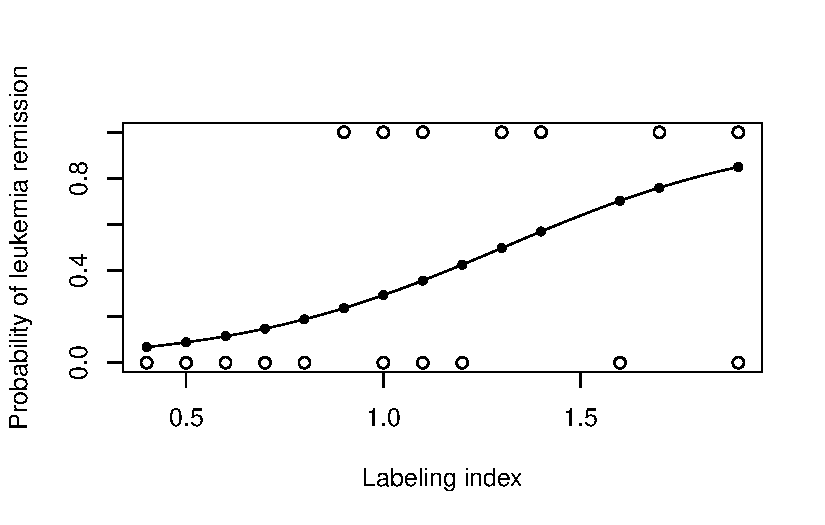
\includegraphics{Metodos_Clasificacion_files/figure-pdf/unnamed-chunk-6-1.pdf}

}

\end{figure}

\hypertarget{los-odds-log-odds-y-odds-ratio}{%
\subsection{Los Odds, Log Odds, y Odds
ratio}\label{los-odds-log-odds-y-odds-ratio}}

El término ``odds'' en estadística y en el contexto de la regresión
logística se refiere a la relación entre la probabilidad de que ocurra
un evento y la probabilidad de que no ocurra. En otras palabras, los
odds representan la proporción de eventos exitosos frente a los eventos
no exitosos.

En la regresión logística, los odds se utilizan para modelar la
probabilidad de que una variable dependiente binaria (por ejemplo, una
variable que toma valores 0 o 1) esté presente o ausente

Existen diversas maneras de escribir la regresión logística, por ejemplo
la primera es.

\[
\frac{\pi}{1-\pi} = exp(\beta_0+\beta_1x_1+\cdots+\beta_{p-1}x_{p-1})
\]

Que es una ecuación, la cual describe la relación entre que ocurra un
evento y no ocurra. Donde \(\pi\) es la probabilidad de que ocurra el
evento. Es decir, si estamos apostando a una carrera de caballos, por
uno en especial gane la carrera, con una probabilidad del 80 porciento,
el \textbf{\emph{odds}}, sería \(0.80/(1-0.80) = 4\) es decir \(4:1\)

La seguna opción es la siguiente:

\[
log(\frac{\pi}{1-\pi}) = \beta_0+\beta_1x_1+\cdots+\beta_{p-1}x_{p-1}
\]

Donde básicamente esta representación nos dice que el logaritmo natural
de los datos, es una función lineal de los datos, y se le conoce como
\textbf{\emph{log odds.}} A esto se le conoce como la
\textbf{\emph{transformación logit}} de la probabilibad de éxito de
\(\pi\)

Por otro lado, el \textbf{\emph{odds ratio}} que lo denominaremos como
\(\theta\) entre los odds de dos predictores, por ejempmplo \(X_{(1)}\)
y \(X_{(2)}\) es dado por :

\[
\theta=\frac{((\pi/(1-\pi))|x=X_{(1)}}{((\pi/(1-\pi))|x=X_{(2)}}
\]

Por otra parte, para una regresión logística los odds de éxito son:

\[
\frac{\pi}{1-\pi} = exp(X\beta)
\]

Es decir, si arreglamos esta ecuación con la anterior, podemos
establecer la relación entre el predictor y la respuesta. El odds ratio
tiene que ser cualquier número no negativo.

Por ejemplo, cuando solo hay un predictor , \(X\) las odds de éxito son

\[
\frac{\pi}{1-\pi} = exp(\beta_0+\beta_1X)
\]

De manera que si incrementamos X por una unidad se convierte en:

\[
\theta = \frac{exp(\beta_0+\beta_1(X+1)}{exp(\beta_0+beta_1X)}=exp(\beta_1)
\]

Por ejemplo, el odds ratio para \texttt{li} se calcula como
\(exp(2.89726)\)

\begin{Shaded}
\begin{Highlighting}[]
\FunctionTok{exp}\NormalTok{(}\FunctionTok{summary}\NormalTok{(lrmodel.reduced)}\SpecialCharTok{$}\NormalTok{coefficients[}\StringTok{"li"}\NormalTok{,}\DecValTok{1}\NormalTok{])}
\end{Highlighting}
\end{Shaded}

\begin{verbatim}
[1] 18.12449
\end{verbatim}

También podemos calcular el intervalo de confianza al 95 porciento como:

\begin{Shaded}
\begin{Highlighting}[]
\FunctionTok{exp}\NormalTok{(}\FunctionTok{summary}\NormalTok{(lrmodel.reduced)}\SpecialCharTok{$}\NormalTok{coefficients[}\StringTok{"li"}\NormalTok{,}\DecValTok{1}\NormalTok{]) }\SpecialCharTok{+}\FunctionTok{qnorm}\NormalTok{(}\FunctionTok{c}\NormalTok{(}\FloatTok{0.025}\NormalTok{,}\FloatTok{0.5}\NormalTok{,}\FloatTok{0.975}\NormalTok{)) }\SpecialCharTok{*} \FunctionTok{summary}\NormalTok{(lrmodel.reduced)}\SpecialCharTok{$}\NormalTok{coefficients[}\StringTok{"li"}\NormalTok{,}\DecValTok{2}\NormalTok{]}
\end{Highlighting}
\end{Shaded}

\begin{verbatim}
[1] 15.79836 18.12449 20.45061
\end{verbatim}

La interpretación del odds ratio es que para cada un incremento de una
unidad en \texttt{li} el estimado de odds para la recurrencia de la
luecemia, está multiplicada por 18.1245. SIn embargo, \texttt{li}
aparece caer entre 0 y 2, por lo que tendría más sentido decir que para
cada incremento en \(0.1\) unidades en \texttt{li}, el estimado de los
odds remission esta multiplicada por \(exp(2.89726\times 0.1) = 1.336\).
Entonces,

\hypertarget{muxe1s-cosas}{%
\subsection{Más cosas \ldots{}}\label{muxe1s-cosas}}

En realidad, cuando estamos tratando con una gran cantidad de datos, no
sería necesario comprobar los supuestos, que básicamente serían los
mismos que los de la regresión multivariada. No obstante, es una buena
práctica hacerlo.

\hypertarget{pruxe1ctica}{%
\section{Práctica}\label{pruxe1ctica}}

\begin{Shaded}
\begin{Highlighting}[]
\FunctionTok{library}\NormalTok{(nnet)}
\FunctionTok{library}\NormalTok{(caret)}
\end{Highlighting}
\end{Shaded}

\begin{verbatim}
Loading required package: ggplot2
\end{verbatim}

\begin{verbatim}
Loading required package: lattice
\end{verbatim}

\begin{Shaded}
\begin{Highlighting}[]
\FunctionTok{set.seed}\NormalTok{(}\DecValTok{123156}\NormalTok{)}
\NormalTok{datos  }\OtherTok{\textless{}{-}} \FunctionTok{read.csv}\NormalTok{(}\StringTok{"./data/BreastTissue.csv"}\NormalTok{)}
\NormalTok{datos}\SpecialCharTok{$}\NormalTok{Class }\OtherTok{\textless{}{-}} \FunctionTok{as.factor}\NormalTok{(datos}\SpecialCharTok{$}\NormalTok{Class)}
\NormalTok{datos[,}\SpecialCharTok{{-}}\DecValTok{1}\NormalTok{] }\OtherTok{\textless{}{-}} \FunctionTok{scale}\NormalTok{(datos[,}\SpecialCharTok{{-}}\DecValTok{1}\NormalTok{])}
\NormalTok{idx }\OtherTok{\textless{}{-}} \FunctionTok{sample}\NormalTok{(}\DecValTok{1}\SpecialCharTok{:}\FunctionTok{nrow}\NormalTok{(datos),}\AttributeTok{size =} \FunctionTok{nrow}\NormalTok{(datos)}\SpecialCharTok{*}\FloatTok{0.7}\NormalTok{,}\AttributeTok{replace =}\NormalTok{ F)}
\NormalTok{train }\OtherTok{\textless{}{-}}\NormalTok{ datos[idx,]}
\NormalTok{test }\OtherTok{\textless{}{-}}\NormalTok{ datos[}\SpecialCharTok{{-}}\NormalTok{idx,]}

\NormalTok{mdl }\OtherTok{\textless{}{-}} \FunctionTok{multinom}\NormalTok{(Class }\SpecialCharTok{\textasciitilde{}}\NormalTok{ ., }\AttributeTok{data =}\NormalTok{ train)}
\end{Highlighting}
\end{Shaded}

\begin{verbatim}
# weights:  66 (50 variable)
initial  value 132.590201 
iter  10 value 50.461488
iter  20 value 38.672193
iter  30 value 36.370299
iter  40 value 34.299155
iter  50 value 33.336058
iter  60 value 32.635862
iter  70 value 30.688927
iter  80 value 28.896317
iter  90 value 28.612742
iter 100 value 28.341508
final  value 28.341508 
stopped after 100 iterations
\end{verbatim}

\begin{Shaded}
\begin{Highlighting}[]
\NormalTok{res }\OtherTok{\textless{}{-}} \FunctionTok{predict}\NormalTok{(mdl,test)}
\end{Highlighting}
\end{Shaded}

\begin{Shaded}
\begin{Highlighting}[]
\FunctionTok{confusionMatrix}\NormalTok{(test}\SpecialCharTok{$}\NormalTok{Class,res)}
\end{Highlighting}
\end{Shaded}

\begin{verbatim}
Confusion Matrix and Statistics

          Reference
Prediction adi car con fad gla mas
       adi   6   0   0   0   0   0
       car   0   7   0   0   0   0
       con   1   0   3   0   0   0
       fad   0   1   0   4   1   0
       gla   0   0   0   0   4   0
       mas   0   1   0   0   2   2

Overall Statistics
                                          
               Accuracy : 0.8125          
                 95% CI : (0.6356, 0.9279)
    No Information Rate : 0.2812          
    P-Value [Acc > NIR] : 6.484e-10       
                                          
                  Kappa : 0.7728          
                                          
 Mcnemar's Test P-Value : NA              

Statistics by Class:

                     Class: adi Class: car Class: con Class: fad Class: gla
Sensitivity              0.8571     0.7778    1.00000     1.0000     0.5714
Specificity              1.0000     1.0000    0.96552     0.9286     1.0000
Pos Pred Value           1.0000     1.0000    0.75000     0.6667     1.0000
Neg Pred Value           0.9615     0.9200    1.00000     1.0000     0.8929
Prevalence               0.2188     0.2812    0.09375     0.1250     0.2188
Detection Rate           0.1875     0.2188    0.09375     0.1250     0.1250
Detection Prevalence     0.1875     0.2188    0.12500     0.1875     0.1250
Balanced Accuracy        0.9286     0.8889    0.98276     0.9643     0.7857
                     Class: mas
Sensitivity              1.0000
Specificity              0.9000
Pos Pred Value           0.4000
Neg Pred Value           1.0000
Prevalence               0.0625
Detection Rate           0.0625
Detection Prevalence     0.1562
Balanced Accuracy        0.9500
\end{verbatim}

\begin{Shaded}
\begin{Highlighting}[]
\FunctionTok{set.seed}\NormalTok{(}\DecValTok{23}\NormalTok{)}
\NormalTok{ctrl }\OtherTok{\textless{}{-}}
  \FunctionTok{trainControl}\NormalTok{(}
    \AttributeTok{method =} \StringTok{"repeatedcv"}\NormalTok{,}
    \AttributeTok{number =} \DecValTok{10}\NormalTok{,}
    \AttributeTok{classProbs =} \ConstantTok{TRUE}\NormalTok{,}
    \AttributeTok{summaryFunction =}\NormalTok{ multiClassSummary}
\NormalTok{  )}
\NormalTok{mdl }\OtherTok{\textless{}{-}} \FunctionTok{train}\NormalTok{(}
  \AttributeTok{x =}\NormalTok{ train[,}\SpecialCharTok{{-}}\DecValTok{1}\NormalTok{],}
  \CommentTok{\# spectral data}
  \AttributeTok{y =}\NormalTok{ train}\SpecialCharTok{$}\NormalTok{Class,}
  \CommentTok{\# factor vector}
  \AttributeTok{method =} \StringTok{"pls"}\NormalTok{,}
  \CommentTok{\# pls{-}da algorithm}
  \AttributeTok{tuneLength =} \DecValTok{10}\NormalTok{,}
  \CommentTok{\# number of components}
  \AttributeTok{trControl =}\NormalTok{ ctrl,}
  \CommentTok{\# ctrl contained cross{-}validation option}
  \AttributeTok{preProc =} \FunctionTok{c}\NormalTok{(}\StringTok{"center"}\NormalTok{, }\StringTok{"scale"}\NormalTok{),}
  \CommentTok{\# the data are centered and scaled}
  \AttributeTok{metric =} \StringTok{"Accuracy"}
\NormalTok{) }\CommentTok{\# metric is ROC for 2 classes}
\end{Highlighting}
\end{Shaded}

\begin{verbatim}
Warning in nominalTrainWorkflow(x = x, y = y, wts = weights, info = trainInfo,
: There were missing values in resampled performance measures.
\end{verbatim}

\begin{Shaded}
\begin{Highlighting}[]
\NormalTok{plsda}
\end{Highlighting}
\end{Shaded}

\begin{verbatim}
function (x, ...) 
UseMethod("plsda")
<bytecode: 0x0000016313462090>
<environment: namespace:caret>
\end{verbatim}

\begin{Shaded}
\begin{Highlighting}[]
\NormalTok{res }\OtherTok{\textless{}{-}} \FunctionTok{predict}\NormalTok{(mdl,test)}
\FunctionTok{confusionMatrix}\NormalTok{(test}\SpecialCharTok{$}\NormalTok{Class,res)}
\end{Highlighting}
\end{Shaded}

\begin{verbatim}
Confusion Matrix and Statistics

          Reference
Prediction adi car con fad gla mas
       adi   6   0   0   0   0   0
       car   0   7   0   0   0   0
       con   1   0   3   0   0   0
       fad   0   1   0   3   1   1
       gla   0   0   0   1   3   0
       mas   0   2   0   2   1   0

Overall Statistics
                                          
               Accuracy : 0.6875          
                 95% CI : (0.4999, 0.8388)
    No Information Rate : 0.3125          
    P-Value [Acc > NIR] : 1.45e-05        
                                          
                  Kappa : 0.6186          
                                          
 Mcnemar's Test P-Value : NA              

Statistics by Class:

                     Class: adi Class: car Class: con Class: fad Class: gla
Sensitivity              0.8571     0.7000    1.00000    0.50000    0.60000
Specificity              1.0000     1.0000    0.96552    0.88462    0.96296
Pos Pred Value           1.0000     1.0000    0.75000    0.50000    0.75000
Neg Pred Value           0.9615     0.8800    1.00000    0.88462    0.92857
Prevalence               0.2188     0.3125    0.09375    0.18750    0.15625
Detection Rate           0.1875     0.2188    0.09375    0.09375    0.09375
Detection Prevalence     0.1875     0.2188    0.12500    0.18750    0.12500
Balanced Accuracy        0.9286     0.8500    0.98276    0.69231    0.78148
                     Class: mas
Sensitivity             0.00000
Specificity             0.83871
Pos Pred Value          0.00000
Neg Pred Value          0.96296
Prevalence              0.03125
Detection Rate          0.00000
Detection Prevalence    0.15625
Balanced Accuracy       0.41935
\end{verbatim}



\end{document}
